%%%%%%%%%%%%%%%%%%%%%%%%%%%%%%%%%%%%%%
% One Column
%%%%%%%%%%%%%%%%%%%%%%%%%%%%%%%%%%%%%%
 \documentclass[smallabstract,smallcaptions]{dccpaper}

\usepackage{epsfig}
\usepackage{epstopdf}
\usepackage{citesort}
\usepackage{amsmath}
\usepackage{amssymb}
\usepackage{color}
\usepackage{url}

\newlength{\figurewidth}
\newlength{\smallfigurewidth}


%%%%%%%%%%%%%%%%%%%%%%%%%%%%%%%%%%%%%%
% One Column
%%%%%%%%%%%%%%%%%%%%%%%%%%%%%%%%%%%%%%
\setlength{\smallfigurewidth}{2.75in}
\setlength{\figurewidth}{6in}

\begin{document}

\title
{\large
\textbf{Template for DCC Manuscripts}
}


\author{%
Author One$^{\ast}$, Author Two$^{\dag}$, and Author Three$^{\ast}$\\[0.5em]
{\small\begin{minipage}{\linewidth}\begin{center}
\begin{tabular}{ccc}
$^{\ast}$Institution One & \hspace*{0.5in} & $^{\dag}$Institution Two \\
Street Address One && Street Address Two \\
City, State, ZIP, Country && City, State, ZIP, Country\\
\url{email@address} && \url{email@address}
\end{tabular}
\end{center}\end{minipage}}
}


\maketitle
\thispagestyle{empty}


\begin{abstract}
The abstract describes concisely and clearly the main contributions of
the paper. It should not contain math equations or citations, to ensure the
abstract is self-contained and readable if converted to ASCII text.
The abstract should contain about 100 to 150 words.
\end{abstract}

\Section{Introduction}

This document follows formatting specified in the \textit{DCC Call for Papers};
top margin 1 inch, left margin 1.25 inches, text area 9 inches high by
6 inches wide, single-column, 12 point type. Submissions in response
to the DCC call may not be more than 10 pages (including all figures,
tables, and appendices).

\Section{Headings}

The \LaTeX class for DCC includes formatting for sections \dots

\SubSection{A Subsection Heading}

and also for subsections. The use of sub-subsections is discouraged.

\Section{Figures and Tables}

The proceedings are published in black and white; all figures and
charts should be clear when printed in grayscale. Figures and tables
should be concise and easy to read. Avoid making complex graphics and
then reducing them so much that they become hard to read.

Position illustrations at the top of the page rather than in the middle
or at the bottom. Caption and number every illustration.
Fig.~\ref{fig:example} shows an example illustration.
Table~\ref{tab:example} shows an example table.


\begin{figure}[t]
\begin{center}
\begin{tabular}{cc}
\multicolumn{2}{c}{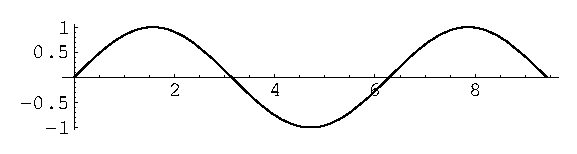
\epsfig{width=4in,file=Figures/image1}} \\
\multicolumn{2}{c}{\small{(a)}} \\[1em]
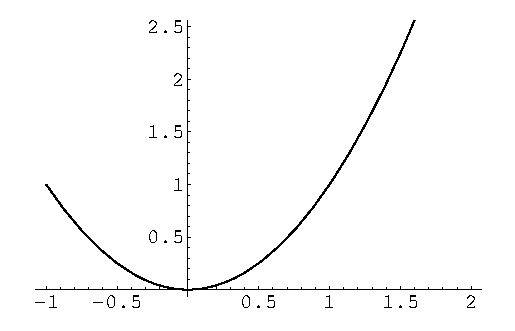
\epsfig{width=2in,file=Figures/image3.eps} &
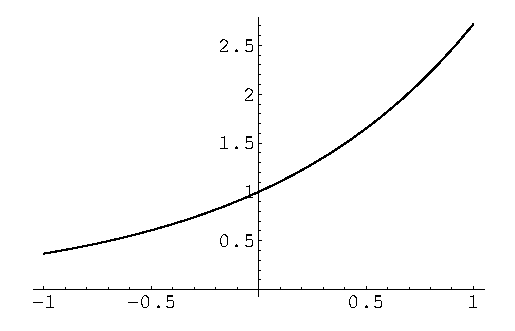
\epsfig{width=2in,file=Figures/image4.eps} \\
{\small (b)} & {\small (c)}
\end{tabular}
\end{center}
\caption{\label{fig:example}%
An example figure.}
\end{figure}

\begin{table}[tp]
\begin{center}
\caption{\label{tab:example}%
Average PSNR in dB for the ``Coastguard'' video sequence}
{
\renewcommand{\baselinestretch}{1}\footnotesize
\begin{tabular}{|c|c|c|c|c|}
\cline{2-5}
\multicolumn{1}{c|}{~}&
\multicolumn{1}{c|}{2D} &
\multicolumn{1}{c|}{3D} &
\multicolumn{2}{c|}{MC-BCS-SPL}\\
\cline{4-5}
\multicolumn{1}{c|}{$S_{\text{NK}}$} &
BCS-SPL & BCS-SPL & $S_{\text{K}}=S_{\text{NK}}$ & $S_{\text{K}}=0.7$\\
\hline
0.1 &22.69 &22.76 &23.06 &25.29 \\
0.2 &24.70 &24.76 &25.78 &27.94 \\
0.3 &26.37 &26.45 &28.29 &30.15 \\
0.4 &27.99 &27.95 &30.88 &32.30 \\
0.5 &29.60 &29.57 &33.58 &34.42 \\
\hline
\end{tabular}}
\end{center}
\end{table}

\Section{Reference to Prior Literature}

List and number all bibliographical references at the end of the
paper. The references can be numbered in alphabetic order or in
order of appearance in the document. When referring to them in
the text, type the corresponding reference number in square
brackets as shown at the end of this sentence \cite{Fow2009}.
The reference list below shows an example of citing a
journal article \cite{Fow2009}, a conference paper \cite{Fow2008},
a book chapter \cite{FD2011}, and a book \cite{Par1998}.
Add your citations to the \url{refs.bib} file.

\Section{References}
\bibliographystyle{IEEEtran}
\bibliography{refs}


\end{document}
